\documentclass[a4paper,12pt]{article}
\usepackage{fontspec}
\setmainfont{Times New Roman}
\setmonofont{DejaVu Sans Mono}[Scale=0.82]
\usepackage[top=3cm,bottom=3.5cm,left=3.5cm,right=2cm]{geometry}
\usepackage[table]{xcolor}
\usepackage{setspace,amsmath,array,booktabs,tabularx,xltabular,enumitem,tikz,xurl,unicode-math}
\setmathfont{Latin Modern Math}
\usetikzlibrary{arrows.meta}
\usepackage{titlesec}
\usepackage{cite}
\usepackage{caption}
\usepackage[unicode,hidelinks]{hyperref}
\urlstyle{same}
\hypersetup{pdftitle={N01 - Đặc tả đề tài và kế hoạch 13 tuần (M0)},pdfauthor={Phan Chí Kiên; Hồ Nhật Khanh}}
\renewcommand{\refname}{Tài liệu tham khảo}
\renewcommand{\tablename}{Bảng}
\renewcommand{\figurename}{Hình}
\makeatletter
\renewcommand\normalsize{\@setfontsize\normalsize{13}{16}}
\makeatother
\AtBeginDocument{\normalsize\onehalfspacing
 \setlength{\abovedisplayskip}{2pt}\setlength{\belowdisplayskip}{2pt}}
\setlength{\parindent}{1cm}
\setlength{\parskip}{0pt}
\setlength{\emergencystretch}{3em}
\setlength{\tabcolsep}{3.5pt}
\setlength{\LTpre}{2pt}
\setlength{\LTpost}{2pt}
\setlist{nosep,leftmargin=1.4em}
\titleformat{\section}{\normalsize\bfseries}{\thesection.}{0.5em}{}
\titlespacing*{\section}{0pt}{3pt}{0pt}
\captionsetup{font={normalsize,stretch=0.94},labelfont=bf,labelsep=colon,skip=3pt}
\newcolumntype{L}[1]{>{\raggedright\arraybackslash}p{#1}}
\renewcommand{\tabularxcolumn}[1]{>{\raggedright\arraybackslash}p{#1}}
% Phần văn bản: Times New Roman 13pt, \onehalfspacing.
% Bảng, chú thích, tài liệu tham khảo: vẫn 13pt, giãn dòng đơn
% (15pt ≈ 1,15 cỡ chữ, tương đương "Single" của Word).
\newcommand{\tblfont}{\setstretch{0.94}\normalsize}
\newcommand{\code}[1]{\texttt{#1}}
\newcommand{\thead}[3]{\toprule \textbf{#1} & \textbf{#2} & \textbf{#3}\\\midrule}
\begin{document}
\begin{center}\setstretch{1.0}
\textbf{ĐẶC TẢ ĐỀ TÀI VÀ KẾ HOẠCH 13 TUẦN (M0)}\\
\textbf{PHÁT TRIỂN THUẬT TOÁN BAY KHÔNG GPS CHO DRONE}\\
Phan Chí Kiên (23520804), Hồ Nhật Khanh (23520716)\\
\end{center}

\section{Thông tin nhóm và đề tài}
Nhóm N01 thực hiện đề tài trong Đồ án 1 (CE201), HK1 2026--2027. Theo mô tả của GVHD~\cite{assignment}, hướng cụ thể là giữ vị trí và bay waypoint trong nhà bằng optical flow và cảm biến khoảng cách, hợp nhất bằng EKF, kiểm chứng trên \textbf{SITL} trước khi bay thật.

\section{Bài toán và mục tiêu}
Trong nhà, tín hiệu GPS yếu hoặc mất nên drone không tự giữ được vị trí. Đề tài giải quyết bài toán ước lượng vị trí, vận tốc cục bộ chỉ bằng cảm biến trên drone. Kết quả phục vụ Lab, dùng chung môi trường mô phỏng với nhóm N02 và làm nền cho Đồ án 2 (CE206). \textbf{Optical flow} là camera nhỏ hướng xuống, đo chuyển động của mặt sàn dưới dạng góc (rad); \textbf{rangefinder} đo khoảng cách xuống sàn để đổi góc đó ra mét~\cite{flow}. Bộ lọc Kalman mở rộng (\textbf{EKF}) hợp nhất hai nguồn này với IMU của flight controller (FC); PX4 có sẵn bộ lọc này (module EKF2)~\cite{ekf}. Nhóm đặt ra bốn mục tiêu:
\begin{enumerate}
\item Khảo sát, so sánh các giải pháp, sản phẩm và nghiên cứu trong, ngoài nước.
\item Làm chủ luồng ước lượng không GPS của EKF2, kiểm chứng trên SITL.
\item Hiện thực thử nghiệm chương trình bay và module giám sát đề xuất (Mục~5).
\item Đo sai số bằng \textbf{ground truth} (GT, vị trí đo độc lập); thử bay thật khi đủ an toàn.
\end{enumerate}

\section{Input -- Output}
Tần số trong Bảng~\ref{tab:io} là giá trị thiết kế dự kiến, chưa đo, không phải mức PX4 bắt buộc; tần số thực tế sẽ được đo trong tuần 2--4. Ở chế độ \textbf{Offboard}, PX4 nhận setpoint (điểm đặt) từ chương trình bên ngoài qua MAVLink và cần setpoint được gửi liên tục~\cite{offboard}. Vị trí theo hệ local NED: gốc tại điểm cất cánh, X Bắc, Y Đông, Z xuống. Dữ liệu cảm biến vào EKF2 qua uORB, kênh thông điệp nội bộ của PX4.

\begingroup\tblfont
\begin{xltabular}{\linewidth}{L{2.6cm}XL{3.0cm}}
\caption{Luồng vào/ra và tần số dự kiến}\label{tab:io}\\
\thead{Luồng}{Nội dung, định dạng, đơn vị}{Tần số}
\endfirsthead
\thead{Luồng}{Nội dung, định dạng, đơn vị}{Tần số}
\endhead
Cảm biến IMU & uORB \code{sensor\_combined}: gia tốc (m/s²), tốc độ góc (rad/s), thời gian (µs). & 100--250 Hz\\
Cảm biến flow & uORB \code{vehicle\_optical\_flow}: góc tích phân (rad), thời gian tích phân (µs), chất lượng 0--255. & 20--50 Hz\\
Cảm biến range & uORB \code{distance\_sensor}: khoảng cách (m), giới hạn min/max (m), chất lượng. & 10--30 Hz\\
Setpoint (vào) & MAVSDK-Python, Offboard: vị trí đặt NED (m), yaw (độ). & 10--20 Hz (PX4 cần trên 2 Hz)\\
Telemetry (ra) & \code{position\_velocity\_ned}: vị trí (m), vận tốc (m/s) ước lượng. & 10--20 Hz\\
Log, GT (ra) & ULog của PX4; CSV thời gian (s), x, y, z (m) của GT; đồ thị sai số, video. & GT từ 30 Hz\\\bottomrule
\end{xltabular}
\endgroup

\section{Phạm vi}
\textbf{Nhóm thực hiện:} khảo sát; cấu hình EKF2 ở chế độ không GPS; chương trình giữ vị trí (hover) và bay hình vuông 2×2~m; module giám sát; công cụ đo sai số; kiểm tra trên bàn; hover thật ở độ cao thấp có bảo hộ nếu đủ điều kiện. \textbf{Nhóm không thực hiện:} viết lại EKF hay bộ điều khiển; phát triển song song trên PX4 và ArduPilot; SLAM, VIO, tránh vật cản, AI; thiết kế FC mới; bay ngoài trời.

\section{Sơ đồ khối và giải pháp đề xuất}
\begin{figure}[ht]
\centering
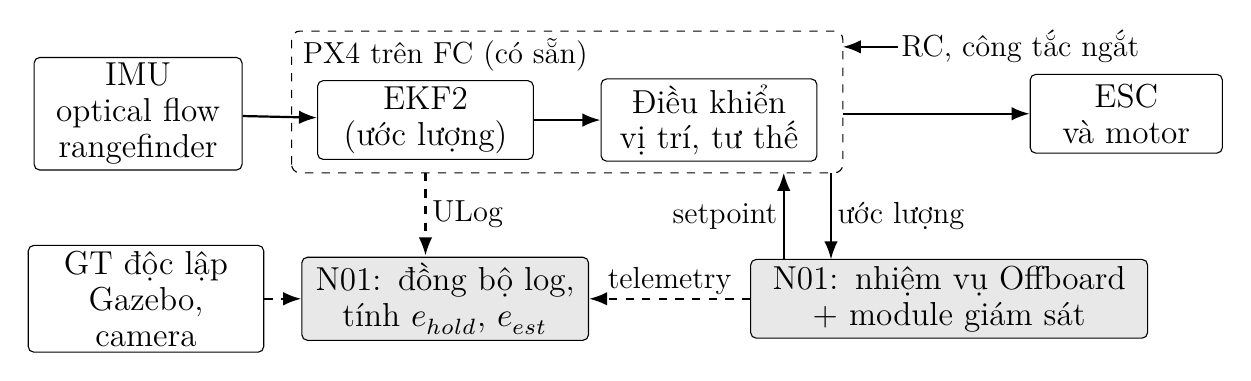
\begin{tikzpicture}[font=\fontsize{12}{13}\selectfont,
 box/.style={draw,rounded corners=2pt,align=center,minimum height=1.0cm,inner sep=2pt},
 own/.style={box,fill=gray!18},
 arr/.style={-{Latex[length=2.3mm]},thick},
 ev/.style={arr,dashed},
 lab/.style={font=\fontsize{11}{12}\selectfont,align=center,inner sep=1pt}]
\draw[dashed,rounded corners=3pt] (3.3,-0.75) rectangle (10.3,1.05);
\node[lab,anchor=north west] at (3.4,1.0) {PX4 trên FC (có sẵn)};
\node[box,text width=2.5cm] (s) at (1.35,0) {IMU\\optical flow\\rangefinder};
\node[box,text width=2.6cm] (e) at (5.0,-0.08) {EKF2\\(ước lượng)};
\node[box,text width=2.6cm] (c) at (8.6,-0.08) {Điều khiển\\vị trí, tư thế};
\node[box,text width=2.3cm] (m) at (13.9,0) {ESC\\và motor};
\node[lab,anchor=west] (rc) at (11.0,0.85) {RC, công tắc ngắt};
\node[box,text width=2.85cm] (g) at (1.45,-2.35) {GT độc lập\\Gazebo, camera};
\node[own,text width=3.5cm] (a) at (5.25,-2.35) {N01: đồng bộ log,\\tính $e_{hold}$, $e_{est}$};
\node[own,text width=4.9cm] (n) at (11.65,-2.35) {N01: nhiệm vụ Offboard\\+ module giám sát};
\draw[arr] (s) -- (e);
\draw[arr] (e) -- (c);
\draw[arr] (10.3,0) -- (m);
\draw[arr] (rc.west) -- (10.3,0.85);
\draw[arr] (9.55,-1.85) -- node[lab,left,xshift=-1pt] {setpoint} (9.55,-0.75);
\draw[arr] (10.15,-0.75) -- node[lab,right,xshift=1pt] {ước lượng} (10.15,-1.85);
\draw[ev] (g) -- (a);
\draw[ev] (5.0,-0.75) -- node[lab,right,xshift=1pt] {ULog} (5.0,-1.8);
\draw[ev] (n) -- node[lab,above] {telemetry} (a);
\end{tikzpicture}
\caption{Sơ đồ khối. Nền xám: phần nhóm làm; nét đứt: luồng đánh giá, GT không đi vào EKF2 hay bộ điều khiển. Trong SITL, Gazebo mô phỏng cảm biến và motor.}\label{fig:system}
\end{figure}

Phần có sẵn của PX4 (khung nét đứt) gồm EKF2, bộ điều khiển, kiểm tra trước khi arm (prearm) và failsafe. \textbf{Module giám sát (đề xuất, cần GVHD xác nhận)} đọc độ hợp lệ của ước lượng, chất lượng flow, range và độ trễ dữ liệu để bay bình thường, giảm tốc khi dữ liệu kém, hoặc dừng và hạ cánh tại chỗ khi mất điều kiện an toàn. Module không thay đổi EKF2 nên không phải một bộ lọc mới. Ngưỡng chọn từ dữ liệu hiệu chuẩn rồi giữ cố định; nhóm so sánh với baseline (cùng cấu hình, không bật module) và báo cáo cả kết quả không đạt.

\section{Tiêu chí đạt và cách đo tại M4}
Nhóm giữ nguyên tiêu chí đạt trong mô tả đề tài~\cite{assignment}: giữ vị trí sai lệch ≤±0,5~m trong 30~s ở độ cao 1--1,5~m; bay 4 waypoint hình vuông 2×2~m; có log so sánh với ground truth. Trên cùng hệ trục và mốc thời gian, gọi $p_{sp}$ là vị trí đặt, $\hat p$ là vị trí ước lượng của EKF2, $p_{GT}$ là vị trí GT; chỉ số $xy$ là thành phần ngang:
\[
e_{hold}(t)=\big\|p_{GT,xy}(t)-p_{sp,xy}\big\|_2,\qquad e_{est}(t)=\big\|\hat p_{xy}(t)-p_{GT,xy}(t)\big\|_2 .
\]
$e_{hold}$ là sai số giữ vị trí của cả hệ, tính bằng GT vì ước lượng có thể trôi cùng drone; $e_{est}$ là sai số của bộ ước lượng. \textbf{Cách hiểu đề xuất, chưa được duyệt:} đạt khi $\max_t e_{hold}\le 0{,}5$~m trong cửa sổ 30~s. Nếu GVHD hiểu “±” theo từng trục, nhóm dùng $\max|\Delta x|$, $\max|\Delta y|$ trong Bảng~\ref{tab:kpi}.

\begingroup\tblfont
\begin{xltabular}{\linewidth}{L{2.3cm}XL{6.4cm}}
\caption{Số liệu đo tại M4 và cách đo}\label{tab:kpi}\\
\thead{Tiêu chí}{Số liệu báo cáo}{Cách đo}
\endfirsthead
\thead{Tiêu chí}{Số liệu báo cáo}{Cách đo}
\endhead
Giữ vị trí & $\max e_{hold}$, $\max|\Delta x|$, $\max|\Delta y|$, RMSE, P95; sai số độ cao. & ≥3 lần ở mỗi độ cao 1,0 và 1,5~m; cách chọn cửa sổ 30~s chốt trước.\\
Hình vuông & Sai số 4 đỉnh, lệch cạnh, thời gian, tỷ lệ hoàn thành. & Qua 4 đỉnh rồi về điểm đầu; tốc độ, ngưỡng waypoint chốt với GVHD.\\
Log và GT & $e_{est}(t)$, mẫu GT thiếu; thiếu GT thì chưa kết luận đạt. & GT từ pose Gazebo hoặc camera, marker; kiểm hệ trục, độ trễ trước khi tính.\\\bottomrule
\end{xltabular}
\endgroup

\section{Thiết bị và phần mềm}
\begingroup\tblfont
\begin{xltabular}{\linewidth}{L{2.35cm}XL{3.2cm}}
\caption{Thiết bị, phần mềm và trạng thái}\label{tab:equipment}\\
\thead{Trạng thái}{Hạng mục (số lượng)}{Ghi chú}
\endfirsthead
\thead{Trạng thái}{Hạng mục (số lượng)}{Ghi chú}
\endhead
Đã có & Mô tả đề tài, khảo sát sơ bộ, kiến trúc dự kiến. & Chưa chạy thử.\\
Chưa xác nhận & PC chạy SITL (1); PX4, Gazebo Harmonic, MAVSDK-Python dùng chung với N02. & Phiên bản chưa khóa.\\
Cần mượn & FC Pixhawk, khung, motor, ESC, bảo vệ cánh (1 bộ); optical flow, vd PMW3901 (1); rangefinder, vd VL53L1X (1). & Cần kiểm driver, nguồn, hướng lắp.\\
Cần mượn & RC có công tắc ngắt, pin, sạc (1 bộ); khu bay có lưới; camera, marker, thước cho GT (1 bộ). & Cần người lái có kinh nghiệm.\\
Cần mua & Giấy hoặc thảm hoa văn trải sàn, in marker; module khác chỉ mua khi Lab không có. & Chờ Lab xác nhận.\\\bottomrule
\end{xltabular}
\endgroup

\section{Kế hoạch 13 tuần và phân công}
Phân công dưới đây là phương án đề xuất, hai thành viên chưa chốt; nếu có điều chỉnh, nhóm sẽ báo GVHD ở M1. Kiên phụ trách ước lượng và EKF2, module giám sát, tích hợp phần mềm. Khanh phụ trách cảm biến, GT và log, phần cứng, kiểm thử. Hai thành viên cùng viết báo cáo và kiểm tra chéo kết quả của nhau.

\begingroup\tblfont\rowcolors{2}{gray!10}{}
\begin{xltabular}{\linewidth}{L{2.35cm}XXL{3.7cm}}
\hiderowcolors\caption{Kế hoạch 13 tuần năm 2026; tuần 2--3 là giai đoạn khảo sát}\label{tab:plan}\\
\toprule \textbf{Tuần} & \textbf{Kiên} & \textbf{Khanh} & \textbf{Đầu ra, mốc}\\\midrule
\endfirsthead
\hiderowcolors\toprule \textbf{Tuần} & \textbf{Kiên} & \textbf{Khanh} & \textbf{Đầu ra, mốc}\\\midrule
\endhead
\showrowcolors
W01\newline28/09--04/10 & Đặc tả, sơ đồ khối, liên hệ N02 & Tiêu chí đo, danh mục thiết bị & M0 (05/10): bản đặc tả\\
W02\newline05/10--11/10 & Khảo sát OF, EKF; chốt bản PX4 với N02 & Khảo sát cảm biến, nguồn trong nước & Phiếu đọc, nhật ký cài đặt\\
W03\newline12/10--18/10 & So sánh giải pháp ước lượng & So sánh cảm biến, cách đo GT & M1 (19/10): khảo sát ≥8 tài liệu\\
W04\newline19/10--25/10 & Baseline không GPS trên SITL & Xuất GT, đồng bộ log & Baseline, log đầu tiên\\
W05\newline26/10--01/11 & Nhiệm vụ Offboard, module giám sát & Script tính sai số, kịch bản lỗi & Module, kịch bản thử\\
W06\newline02/11--08/11 & Tích hợp, lý giải giải pháp & Chạy thử, video, Git & M2 (09/11): báo cáo, video, Git\\
W07\newline09/11--15/11 & Đối chứng module với baseline & Nhận, kiểm thiết bị mượn & Bảng đối chứng SITL\\
W08\newline16/11--22/11 & Cấu hình tham số cho phần cứng & Kiểm tra tháo cánh, camera GT & Checklist kiểm tra trên bàn\\
W09\newline23/11--29/11 & Prototype luồng chính & Kiểm thử, danh sách lỗi & M3 (30/11): báo cáo, video, Git\\
W10\newline30/11--06/12 & Vận hành phần mềm khi thử hover (Mục~9) & Quan sát, ghi GT, video & Dữ liệu hover hoặc báo cáo vướng mắc\\
W11\newline07/12--13/12 & Phân tích sai số, đối chiếu khảo sát & Đo theo tiêu chí, bảng số liệu & M4 (14/12): số liệu, bản nháp\\
W12\newline14/12--20/12 & Hoàn thiện mã, phân tích & Kiểm tra tái hiện theo hướng dẫn & Gói mã, hướng dẫn chạy\\
W13\newline21/12--27/12 & Phần thuật toán, slide & Phần thực nghiệm, video & M5 (28/12): báo cáo, slide, video\\\bottomrule
\end{xltabular}
\endgroup

\section{Rủi ro, an toàn và dự phòng}
\begingroup\tblfont
\begin{xltabular}{\linewidth}{L{5.6cm}XL{1.9cm}}
\caption{Rủi ro chính và phương án dự phòng}\label{tab:risk}\\
\thead{Rủi ro}{Dự phòng}{Theo dõi}
\endfirsthead
\thead{Rủi ro}{Dự phòng}{Theo dõi}
\endhead
Lệch phiên bản, model lỗi & Khóa phiên bản, thử sớm từ tuần 2 & Kiên\\
Trôi do sàn ít vân, range sai & Trải sàn hoa văn; dừng khi mất hợp lệ & Kiên\\
GT sai hệ trục, trễ, thị sai & Kiểm bằng dịch chuyển biết trước & Khanh\\
Thiếu thiết bị hoặc khu bay & Mượn từ tuần 2; báo GVHD trước M3 & Khanh\\
Module không hơn baseline & Báo cáo và phân tích nguyên nhân & Kiên\\\bottomrule
\end{xltabular}
\endgroup

\textbf{Bốn bước an toàn} theo thứ tự: (1) SITL: tắt GPS, hợp nhất flow và range, vị trí local hợp lệ; (2) kiểm tra trên bàn, tháo cánh: nguồn, cảm biến, RC, công tắc ngắt, motor; (3) hover thấp có lưới hoặc dây, người lái đủ năng lực, người quan sát, RC độc lập với chương trình nhóm; (4) hình vuông thật khi hover ổn định, khu bay đủ rộng. Không bỏ prearm check, không dùng RTL (tự quay về) trong nhà, không tạo lỗi cảm biến khi bay thật. SITL không thay bay thật; thiếu điều kiện thì báo GVHD.

\textbf{Nhóm đề nghị GVHD cho ý kiến về:} cách hiểu “±0,5~m”, ngưỡng waypoint, vai trò module giám sát, thiết bị, khu bay. Nhóm chưa chạy SITL, chưa bay thật.

\section{Nguồn dự kiến khảo sát và tài liệu tham khảo}
Tuần 2--3, nhóm đọc, so sánh ít nhất 8 tài liệu theo cảm biến, độ trôi, điều kiện thử, cách đo GT, chi phí. Hiện có: bài báo nước ngoài~\cite{gageik,wang,honegger,grabe}, nghiên cứu trong nước~\cite{vn}, sản phẩm thương mại~\cite{ark}, tài liệu PX4~\cite{flow,ekf,offboard}; nhóm đang tìm thêm đề tài trong nước.

\begingroup\tblfont\raggedright
\renewcommand{\section}[2]{}%
\begin{thebibliography}{99}
\setlength{\itemsep}{0pt}
\bibitem{assignment} N. D. X. Bách, “Đồ án 1 -- Đồ án 2, HK1 2026--2027: Mô tả đề tài và kế hoạch thực hiện,” Khoa KTMT, Trường ĐH CNTT, email 25/09/2026, tr. 1--3, 12.
\bibitem{flow} PX4 Development Team, “Optical Flow,” \textit{PX4 User Guide}.\newline\url{https://docs.px4.io/main/en/sensor/optical_flow.html} (truy cập 29/09/2026).
\bibitem{ekf} PX4 Development Team, “Using PX4’s Navigation Filter (EKF2),” \textit{PX4 User Guide}. \url{https://docs.px4.io/main/en/advanced_config/tuning_the_ecl_ekf.html} (truy cập 29/09/2026).
\bibitem{offboard} PX4 Development Team, “Offboard Mode,” \textit{PX4 User Guide}.\newline\url{https://docs.px4.io/main/en/flight_modes/offboard.html} (truy cập 29/09/2026).
\bibitem{gageik} N. Gageik, M. Strohmeier, và S. Montenegro, “An autonomous UAV with an optical flow sensor for positioning and navigation,” \textit{Int. J. Adv. Robot. Syst.}, vol. 10, no. 10, 2013, doi: 10.5772/56813.
\bibitem{wang} R. Wang, D. Zou, C. Xu, L. Pei, P. Liu, và W. Yu, “An aerodynamic model-aided state estimator for multi-rotor UAVs,” \textit{Proc. IEEE/RSJ IROS}, 2017, tr. 2164--2170, doi: 10.1109/IROS.2017.8206034.
\bibitem{honegger} D. Honegger, L. Meier, P. Tanskanen, và M. Pollefeys, “An open source and open hardware embedded metric optical flow CMOS camera for indoor and outdoor applications,” \textit{Proc. IEEE ICRA}, 2013, tr. 1736--1741, doi: 10.1109/ICRA.2013.6630805.
\bibitem{grabe} V. Grabe, H. H. Bülthoff, D. Scaramuzza, và P. R. Giordano, “Nonlinear ego-motion estimation from optical flow for online control of a quadrotor UAV,” \textit{Int. J. Robot. Res.}, vol. 34, no. 8, tr. 1114--1135, 2015, doi: 10.1177/0278364915578646.
\bibitem{vn} M. T. Nguyen \textit{và cộng sự}, “Stabilzation position of quadcopter using vision-based corner detector from top-down footage of camera,” \textit{J. Tech. Educ. Sci.}, số 71A, tr. 18--27, 2022, doi: 10.54644/jte.71A.2022.1132.
\bibitem{ark} PX4 Development Team, “ARK Flow,” \textit{PX4 User Guide}, trang sản phẩm.\newline\url{https://docs.px4.io/main/en/dronecan/ark_flow.html} (truy cập 29/09/2026).
\end{thebibliography}
\endgroup
\end{document}
